Der folgende Abschnitt beschreibt die Funktionsweise und den Prozess zur Erstellung der Rolle des Verteidigers.

\subsubsection{Vorgehensweise}
\textit{Verfasser: Weber}\\

\begin{figure}[H]
	\centering
	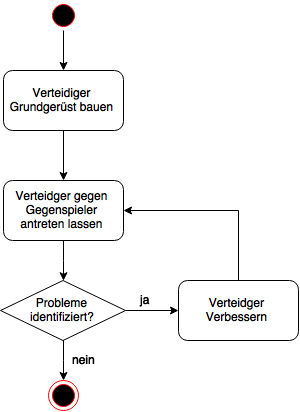
\includegraphics[width=0.5\textwidth]{Grafiken/KI/defender/vorgehensweise.png}
	\caption{Vorgehensweise zur Entwicklung des Verteidigers}
	\label{Vorgehensweise-Verteidigers}
\end{figure}
Der in Abbildung \ref{Vorgehensweise-Verteidigers} dargestellte Prozess ist der Anforderung geschuldet zu einem m"oglichst fr"uhen Zeitpunkt bereits einen funktionierenden Spieler auf das Feld schicken zu k"onnen. Deswegen wurde ein iterativer Prozess gew"ahlt, zu Beginn wird ein einfaches Grundger"ust entwickelt. Dieses wird anschlie"senden zyklisch verbessert. Der Prozess kann verlassen werden, wenn keine Zeit mehr f"ur Verbesserungen vorhanden ist, oder keine weiteren Probleme identifiziert werden k"onnen.

\subsubsection{Use-Cases}
\textit{Verfasser: Weber}\\
\begin{figure}[H]
	\centering
	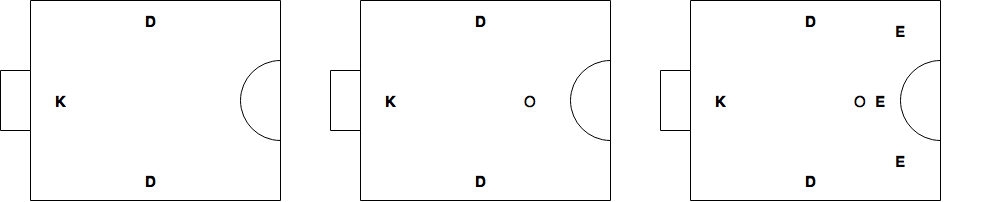
\includegraphics[width=\ScaleIfNeeded]{Grafiken/KI/defender/useCases.png}
	\caption{Die Use-Cases des Verteidigers}
	\label{Usecases-Verteidigers}
\end{figure}

F"ur den Verteidiger wurden die in Abbildung \ref{Usecases-Verteidigers} Use-Cases ermittelt. Die identifizierten Use-Cases hatten nicht den Anspruch alle m"oglichen F"alle abzubilden, sich aber auf einige wenige wichtige zu reduzieren. Bei der Erstellung der Use-Cases wurden mehrere idealisierende Annahme beachtet.

\begin{itemize}
\item Auf dem Spielfeld befinden sich nur Spieler der Rolle Verteidiger.
\item Der Verteidiger bewegt sich in jedenfall genau so schnell wie der Angreifer.
\item Der Verteidiger stellt ein Hindernis dar, welches umlaufen wird.
\end{itemize}

Generell wurde dem gegnerischen Spieler eine h"ohere Priorit"at zugeteilt als dem Ball. Falls der Ball nicht durch den gegnerischen Spieler in das Spielfeld getragen wird, versucht der Gegner den Ball f"ur sich zu erobern. Da die gegnerischen Spieler von dem Verteidiger gedeckt werden, sollten diese gleichzeitig bei dem Ball ankommen.

\paragraph{UseCase D1: Spielgeschehen auf anderer Spielh"alfte}
\label{UseCaseD1}
Weder der Ball noch Gegnerische Spieler befinden sich auf der eigenen Spielh"alfte.
\paragraph{UseCase D2: Ball in eigener Spielh"alfte}
\label{UseCaseD2}
Der Ball jedoch keine gegnerischen Spieler befinden sich auf der eigenen Spielh"alfte.
\paragraph{UseCase D3: Gegner (mit Ball) in eigener Spielh"alfte}
\label{UseCaseD3}
Gegnerische Spieler befinden sich auf dem Spielfeld. Dabei ist es unerheblich ob der Ball ebenfalls mit auf dem Spielfeld ist.

\subsubsection{Klassendiagramm}
\textit{Verfasser: Weber}\\
\begin{figure}[H]
	\centering
	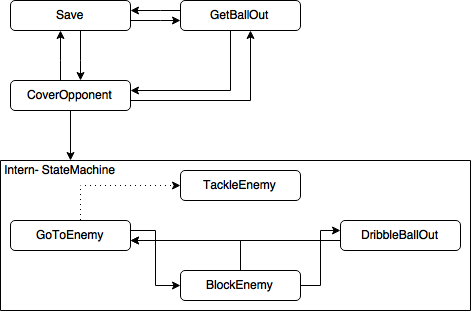
\includegraphics[width=0.8\textwidth]{Grafiken/KI/defender/defender.png}
	\caption{Vorgehensweise zur Entwicklung des Verteidigers}
	\label{Vorgehensweise-Verteidigers}
\end{figure}

Der Verteidiger wurde wie alle Rollen als State-Automat entworfen. Aus den Use-Cases wurden direkt 3 direkte Abbildungen entwickelt \lstinline{Save}, \lstinline{GetBallOut} und \lstinline{CoverOpponent}. Wobei die \lstinline{CoverOpponent}-Klasse noch eine internen State-Automat besitzt. Alle Klassen teilen sich die \lstinline{DefenseBaseState}-Klasse, die eine gewisse Basis-Funktionalit"at zur Verf"ugung stellt.

\paragraph{Save-State}
Der Save-State ist die Abbildung zum UseCase D1. In diesem State positioniert sich der Roboter nur auf seiner Home-Position und "uberwacht das akutelle Spiel auf Ver"anderungen.

\paragraph{GetBallOut-State}
Dient dazu den Ball aus der eigenen Spielfeldh"alfte zu entfernen. Urspr"unglich war dieser State eine exakte Abbildung des UseCases D2. Durch sp"atere Tests wurde die Transition zu diesem State erleichtert, sodass Situationen in denen der ``Ball als frei gilt'' ebenfalls eine Transition ausl"ost.\\
\\
Als frei wird der Ball bezeichnet (in der aktuellen Implementierung), wenn der n"achste Spieler am Ball vom gegnerischen Team und entweder zuweit entfernt oder umgefallen ist.

\paragraph{CoverOpponent-State}
In diesem State, werden ``freie gegnerische Spieler'' auf der eigenen Spielfeldh"alfte erkannt und der interne State-Automat ausgef"uhrt. Dieser bestimmt die exakten Aktionen des Roboters. Die \lstinline{CoverOpponent}-State Klasse ist lediglich daf"ur zust"andig den Gegner mit der h"ochsten Priorit"at zu finden, sollte ein solcher bestimmt worden sein, beginnt die Ausf"uhrung des internen State-Automaten beginnend mit der \lstinline{GoToEnemy}-Klasse.\\
\\
Als frei wird ein gegenerischer Spieler bezeichnet, wenn in seinem direkten Unfeld keine eigenen Spieler existieren, die ihn bereits decken. Sollten mehrere Spieler gefunden welche, dieses Kriterium erf"ullen, wird zuerst der Spieler mit dem Ball gedeckt, danach entscheidet die Distanz zum Tor.

\paragraph{GoToEnemy-State}
In erster Linie dient diese Klasse, wie der Name bereits verr"at, dazu eine Position zwischen dem Feind und dem Tor einzunehmen. Anschlie"send entscheidet die Klasse welche folge Zustand ausgef"uhrt werden soll. Der "Ubergang zu der \lstinline{TackleEnemy}-Klasse wurd im Verlauf der Entwicklung aus der Logik des Roboters entfernt.

\paragraph{TackleEnemy-State}
In dem urspr"unglichen Entwurf, sollte der Verteidiger mit einem gewichteten Zufall entscheiden ob er den Feind nach erreichen der Position, blockiert oder umwirft. Die Gewichtung konnte zum Konstruktionszeitpunkt bestimmt werden. Bei der aggressiven Strategie wurde zum Beispiel, die wahrscheinlichkeit f"ur ein Foul erh"oht. Jedoch wurde dieser State w"ahrend der Entwicklung verworfen, da das ``Tackeln'' sich als unstabil erwies.

\paragraph{BlockEnemy-State}
In dem ersten Entwicklungszyklus des Verteidigers, blockierte er nur den Weg des Verteidigers. Erst in dem Entwicklungsprozess wurde der letzte "Ubergang hinzugef"ugt und die Aufgaben der \lstinline{BlockEnemy} erweitert, sodass sie zus"atzlich darauf achtet ob der ``Gegner den Ball verliert''. Sollte dies der Fall sein, wird der "Ubergang zur \lstinline{DribbleBallOut} Klasse ausgef"uhrt.

\paragraph{DribbleBallOut-State}
Sollte der Roboter sich in diesem State befinden so bedeutet dies, wie bereits erl"autert, dass der Gegner den Ball verloren hat und er nun aus dem Spielfeld gebracht werden muss. Der State sucht nach Hindernissen, und versucht den Ball vor die Mittelfeldbegrenzung zudribbeln. Sollte dies erfolgreich verlaufen sein, schie"st er den Ball zu einem seinen Mitspielern.

\subsubsection{Wahl der Szenarien}
\textit{Verfasser: Weber}\\
Der Verteidiger wurde mit 3 Zyklen evaluiert.

\paragraph{Antritt gegen manuellen Bot}
Testen der "Uberg"ange gegen einen menschlich gesteuerten Roboter.

\paragraph{Antritt gegen SimpleBot}
In den ersten Runden wurde ein gr"osseres Problem entdeckt. Die erste Annahme, das ein Gegner stehen bleibt, war nicht haltbar. Das sich auch bei dem Testspiel mit Team KKB best"atigte. Deswegen wurde in diesem Zyklus die \lstinline{DribbleBallOut} Klasse zu dem internen State-Automat hinzugef"ugt. Bei den Tests wurde auch festgestellt, dass der State \lstinline{TackleEnemy} nicht die gew"unschte Leistung produzierte und wurde verworfen. Einige weitere Stellschrauben waren dar"uber hinaus, das Kriterium zur Erreichen der Position in der \lstinline{GoToEnemy} Klasse, die eigentliche Positions Bestimmung (unter Beruecksichtsnahme der distanz der beiden Roboter), sowie die Kriterien f"ur den "Ubergang von \lstinline{BlockEnemy} auf \lstinline{DribbleBallOut} State.

\paragraph{Antritt gegen St"urmer}
Verbesserungen in diesem Zyklus waren haupts"achlich das der "Ubergang von der \lstinline{CoverOpponent} zur \lstinline{GetBallOut} erleichter wurden. Ebenfalls wurde die \lstinline{DribbleBallOut}-Klasse erweitert, sodass sie nun das Ausweichen von mehreren Gegnern enthielt und den Pass zu eigenen Spielern. Als letzte Ma"snahme wurde der "Ubergang von der \lstinline{BlockEnemy} zur \lstinline{DribbleBallOut} erweitert.



